\lecture{Plant Layout}{24~-~01~-~2026}
%
%
\section{Definizione e obiettivi}
Il Plant Layout è la progettazione della disposizione plano-altimetrica di macchinari, impianti, addetti e materiali all'interno di uno stabilimento. Non si limita alla sola posizione delle macchine, ma comprende la progettazione ottimale di tutti i flussi (manodopera, trasporti interni, servizi accessori) e della struttura edilizia atta a contenerli.

Gli obiettivi principali di un layout ottimale sono:
\begin{itemize}
    \item \textbf{Semplificare il processo produttivo} e ridurre i ritardi;
    \item \textbf{Minimizzare i costi di trasporto} dei materiali e le scorte;
    \item Utilizzare lo spazio e la manodopera nel modo più efficace;
    \item Garantire un ambiente di lavoro sicuro e soddisfacente.
\end{itemize}
Le modifiche al layout si classificano in due categorie:
\begin{enumerate}
    \item \emph{Brown field}: Modifiche o trasformazioni di layout esistenti o trasferimenti in stabilimenti già costruiti.
    \item \emph{Green field}: Costruzione di un nuovo stabilimento da zero.
\end{enumerate}

%
\section{Tipologie di Layout}
La scelta del layout dipende dal volume di produzione e dalla varietà dei prodotti.
Per il confronto dei diversi layout, vedi figura \ref{fig:layout_comparison}.
%
\paragraph{Layout per Prodotto (Line Layout)} Caratteristico delle produzioni di grande serie (es. automobili). Ogni area produce un solo prodotto o prodotti molto simili.
\begin{itemize}
    \item \textbf{Caratteristiche}: Flusso lineare, macchine disposte in sequenza operativa.
    \item \textbf{Vantaggi}: Bassi costi di trasporto, tempi di produzione ridotti, scorte minime, alta produttività, minor superficie richiesta.
    \item \textbf{Condizioni ideali}: Alti volumi, prodotti standardizzati, domanda stabile.
\end{itemize}
Vedi figura \ref{fig:line_layout}.

%
\paragraph{Layout per Processo (Functional / Job Shop)} Riunisce in reparti le lavorazioni dello stesso tipo (es. reparto tornitura, reparto fresatura \dots).
\begin{itemize}
    \item \textbf{Caratteristiche}: Indicato per produzioni in piccoli lotti e alta varietà. Flessibilità elevata.
    \item \textbf{Vantaggi}: Minori investimenti in macchinari (non duplicati), maggiore flessibilità, minore impatto in caso di guasti macchina.
    \item \textbf{Svantaggi}: Maggiori costi di trasporto e tempi di attraversamento più lunghi.
\end{itemize}
Vedi figura \ref{fig:process_layout}.

%
\paragraph{Layout a Punto Fisso} Il prodotto rimane fermo (es. navi, aerei) mentre attrezzature e personale si muovono verso di esso.
\begin{itemize}
    \item \textbf{Utilizzo}: Oggetti voluminosi e pesanti; investimenti di capitale minimi nel layout.
\end{itemize}

%
\paragraph{Layout a Isole (Cellular Layout / Group Technology)} Un approccio ibrido che raggruppa le lavorazioni per ``famiglie'' di prodotti.
\begin{itemize}
    \item \textbf{Struttura}: Celle di lavoro (spesso a forma di U, T, S) dove si completano le lavorazioni su una famiglia di pezzi.
    \item \textbf{Vantaggi}: Riduzione del Lead Time, dello stock e dei flussi intercellulari; miglioramento della qualità e del controllo.
\end{itemize}
Vedi figura \ref{fig:island_layout}.

\begin{figure}
    \centering
    \begin{subfigure}{0.45\linewidth}
        \centering
        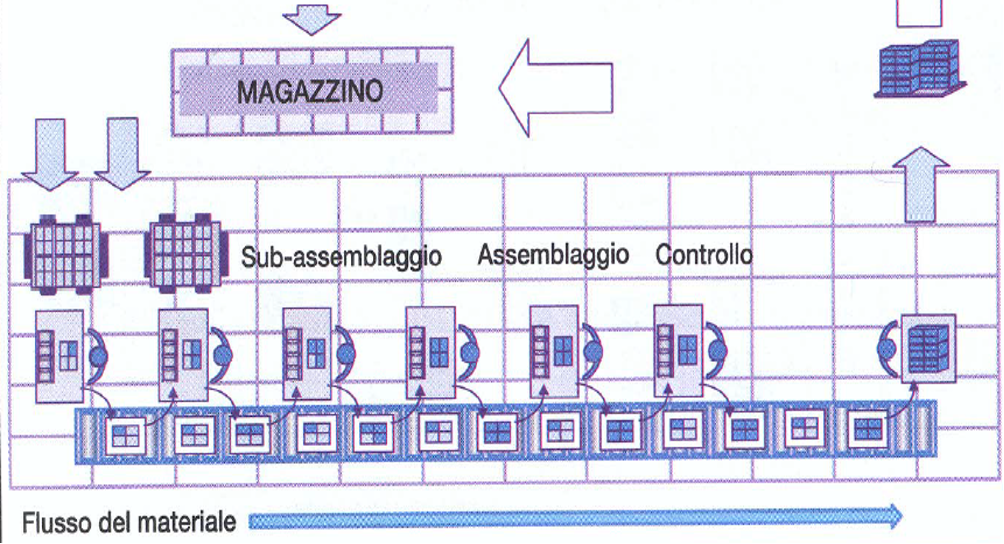
\includegraphics[width=\linewidth]{assets/Picture 1.png}
        \caption{Layout a linea in area di assemblaggio}\label{fig:line_layout}
    \end{subfigure}
    \begin{subfigure}{0.45\linewidth}
        \centering
        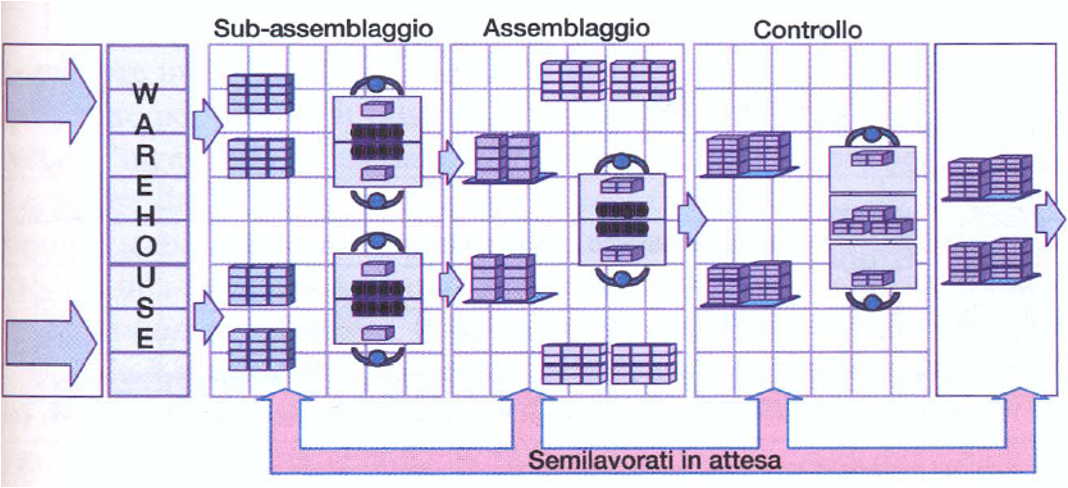
\includegraphics[width=\linewidth]{assets/Picture 2.png}
        \caption{Layout per processo in area di assemblaggio}\label{fig:process_layout}
    \end{subfigure}
    \begin{subfigure}{0.4\linewidth}
        \centering
        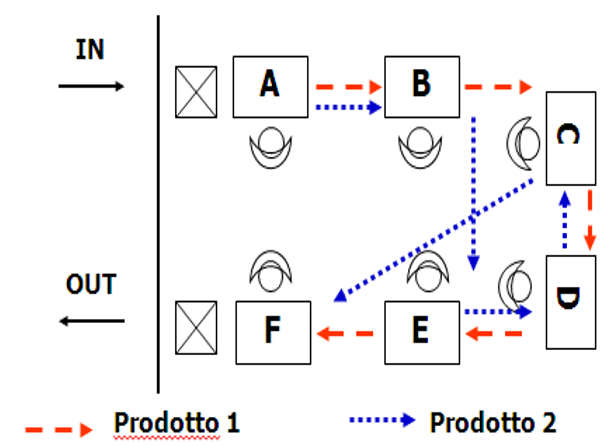
\includegraphics[width=\linewidth]{assets/Picture 3.png}
        \caption{Layout a isole}\label{fig:island_layout}
    \end{subfigure}
    \begin{subfigure}{0.4\linewidth}
        \centering
        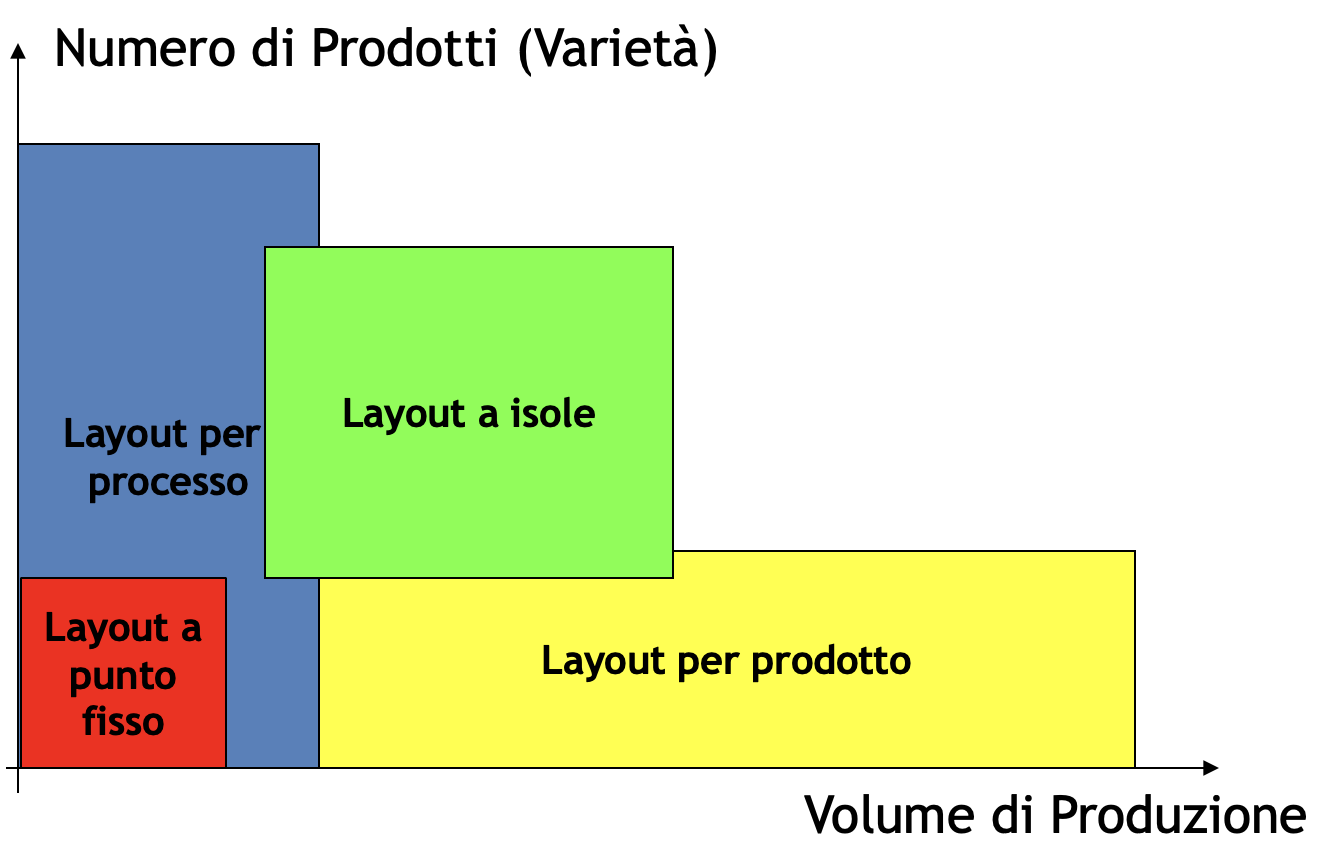
\includegraphics[width=\linewidth]{assets/Screenshot 2026-01-24 at 15.37.56.png}
        \caption{Confronto dei layout. }\label{fig:layout_comparison}
    \end{subfigure}
    \caption{Tipi di layout}
\end{figure}

%
\subsection{Analisi prodotto-quantità}
La scelta del layout dipende dal volume di produzione e dalla varietà dei prodotti. Per analizzare questa relazione si utilizza l'istogramma P-Q (\emph{Analisi ABC}):
\begin{enumerate}
    \item \textbf{Classe A} (Alta quantità, bassa varietà): Layout per prodotto (Linea);
    \item \textbf{Classe B} (Media quantità/varietà): Layout a isole.
    \item \textbf{Classe C} (Bassa quantità, alta varietà): Layout per processo;
\end{enumerate}
Vedi figura \ref{fig:pq_analysis}.
\begin{figure}
    \centering
    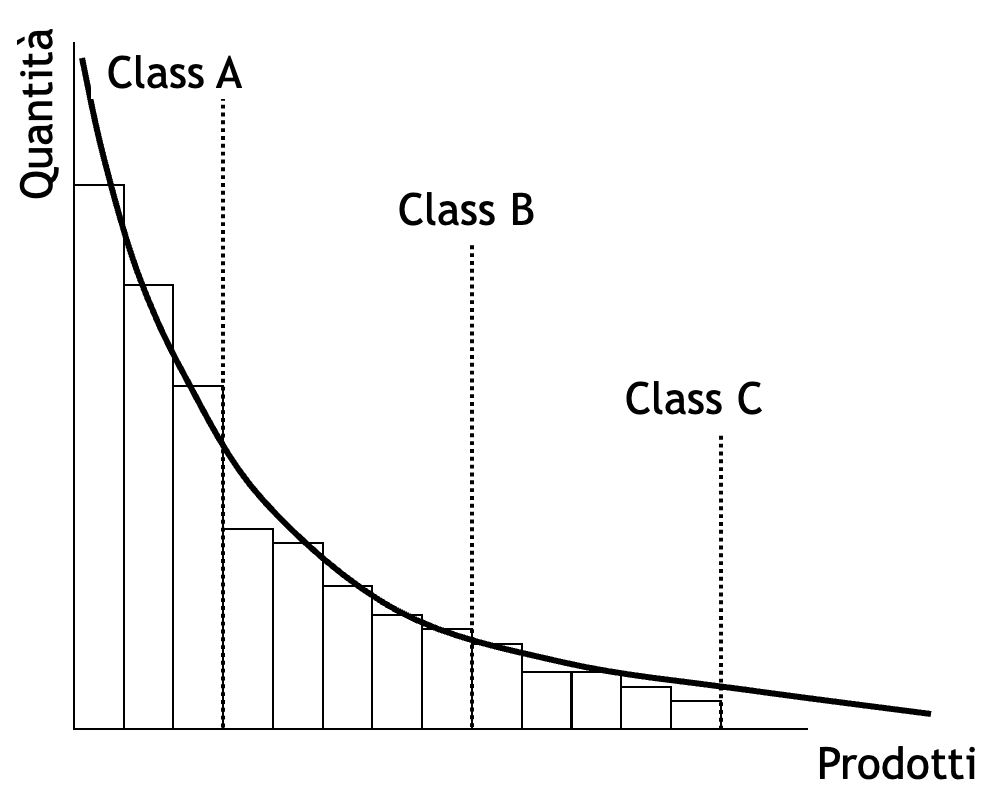
\includegraphics[width=0.4\linewidth]{assets/Screenshot 2026-01-24 at 15.40.55.png}
    \caption{Analisi prodotto-quantità. }\label{fig:pq_analysis}
\end{figure}

%
\section{Progettazione del layout}
Per progettare il layout sono necessari dati precisi: ciclo di lavorazione (Flow Chart), volumi, pesi, tempi e servizi richiesti.

Inoltre, lo studio sistematico delle possibili soluzioni di plant layout viene condotto prendendo in esame:
\begin{enumerate}
    \item i tipi delle lavorazioni;
    \item i possibili sistemi di trasporto interno;
    \item i posti di lavoro.
\end{enumerate}

%
\paragraph{Takt Time e dimensionamento} Il \emph{Takt Time} è il ritmo produttivo necessario per soddisfare la domanda di mercato.
%
\subparagraph{Takt time su intervallo temporale fissato}
\[
    \text{Takt Time} = \frac{\text{Tempo di lavoro disponibile}}{\text{Domanda di mercato}}
\]
\begin{example}
    Abbiamo:
    \begin{itemize}
        \item $ 2\ h $: ore di lavoro;
        \item $ 100\ u$: unità richieste.
    \end{itemize}
    \[
        \text{Takt Time} = \frac{2\ h}{100\ u} = \frac{120\ min}{100\ u}= 1.2\ \frac{min}{u}
    \]
\end{example}
%
\subparagraph{1/Takt time (Quante unità di prodotto al minuto)}
\[
    \text{Takt Time} = \frac{1}{\text{Takt Time}} = \frac{1}{1.2\ \frac{min}{u}} = 0.83\ \frac{u}{min}
\]

%
\subparagraph{Takt Time con rendimento} Se l'impianto ha un rendimento diverso dal 100\%, il tempo disponibile si riduce:
\[
    \text{Tempo di lavoro effettivo} = \text{Tempo di lavoro disponibile} \times \text{Rendimento}
\]
\begin{example}
    \begin{gather*}
        \text{Rendimento} = 80\% \\
        \text{Domanda di mercato} = 1000\ u \\
        \text{Tempo di lavoro disponibile} = 8\ h = 480\ min \\
        \text{Tempo di lavoro effettivo} = 480\ min \times 0.8 = 384\ min \\
        \text{Takt Time} = \frac{384\ min}{1000\ u} = 0.384\ \frac{min}{u}
    \end{gather*}
\end{example}

%
\subparagraph{Takt time con rendimento e scarti} Se sono presenti scarti, il numero di unità da lavorare aumenta:
\[
    \text{Unità da lavorare} = \frac{\text{Numero di unità}}{(1-r_{0})(1-r_{1}) \dots (1-r_{n})}
\]
Dove:
\begin{itemize}
    \item Numero di unità: unità richieste da produrre;
    \item $ r_{n} $: tasso di scarto $ r $ da sottrarre ad 1 per ogni fase di lavorazione $ n $.
\end{itemize}
\begin{example} Ad esempio:
    \begin{itemize}
        \item Numero di unità: $ 1000\ u $;
        \item Tasso di scarto per 3 operazioni: $ r_{0} = 3\% $, $ r_{1} = 2.5\% $, $ r_{3} = 0.5\% $;
    \end{itemize}
    \[
        \text{Unità} = \frac{1000}{(1-0.03)(1-0.025)(1-0.005)} = 1063\ u
    \]
    Da notare, il risultato viene sempre arrotondato per eccesso.
\end{example}
%
%
\paragraph{Pitch time} È il Takt Time moltiplicato per la quantità nel contenitore standard (lotto di movimentazione).
%
\paragraph{Calcolo numero macchine}
\[
    \#\text{macchine} = \frac{\text{Tempo ciclo macchina}}{\text{Takt Time}}
\]
\begin{example}
    Ad esempio:
    \begin{itemize}
        \item Tempo ciclo macchina: $0.5 \frac{min}{u} $;
        \item Domanda media: $ 1000\ u $;
        \item Tempo di lavoro disponibile: $ 8\ h = 480\ min $;
        \item Rendimento impianto: $ 80\% $.
    \end{itemize}
    \begin{gather*}
        \text{Takt time} = \frac{480\ min \cdot 0.8}{1000\ u} = 0.384\ \frac{min}{u} \\
        \#\text{macchine} = \frac{0.5\ \frac{min}{u}}{0.384\ \frac{min}{u}} \approx 2\ \text{macchine}
    \end{gather*}
\end{example}
%
\subsection{Sistemi di trasporto interno} L'obiettivo matematico è minimizzare il costo totale dei trasporti interni. La funzione obiettivo è:
\[
    C = \sum_{i=1}^{N} \sum_{j=1}^{N} T_{ij} \cdot c_{ij} \cdot d_{ij}
\]
dove:
\begin{itemize}
    \item $ C $: costo totale;
    \item $ T_{ij} $: trasferimenti tra la locazione $ i $ e la locazione $ j $;
    \item $ c_{ij} $: costo per unità di distanza e per trasferimento tra $ i $ e $ j $;
    \item $ d_{ij} $: distanza tra la locazione $ i $ e la locazione $ j $;
    \item $ N $: numero totale di locazioni.
\end{itemize}
%
\paragraph{Strumenti di Analisi}
\begin{enumerate}
    \item \textbf{Matrice dei Trasferimenti} (Flow Matrix): Indica la quantità di movimenti tra i reparti;
    \item \textbf{Matrice dei Costi}: Costo per metro per unità di carico;
    \item \textbf{Matrice delle Distanze}: Dipende dalla disposizione fisica ipotizzata.
\end{enumerate}
%
\subsection{Algoritmi e metodi specifici}
Per ottimizzare la disposizione (in particolare nei layout per processo) si usano:
\begin{enumerate}[label=\alph*)] % chktex-file 9 chktex-file 10
    \item Metodo delle Intensità di Traffico;
    \item Metodo di Hollier (o dei Flussi);
    \item Triangolo di Buffa.
\end{enumerate}

\subsubsection{Metodo delle Intensità di Traffico} Si basa sull'avvicinare i reparti che hanno i flussi di materiale più intensi, visualizzando i collegamenti come legami pesati.
\subsubsection{Metodo di Hollier} Utilizzato per disporre le risorse (macchine o reparti) in sequenza lineare minimizzando i ritorni (``backtracking''). Procedura:
\begin{enumerate}
    \item Costruire la tabella ``From/To'' dei flussi;
    \item Calcolare per ogni macchina il totale dei flussi in uscita (``from'') e in entrata (``to''), vedi figura \ref{fig:fromto_matrix};
    \item Calcolare il rapporto $r=\frac{\text{From}}{\text{To}}$ per ogni risorsa, vedi figura \ref{fig:ratio_matrix};
    \item Ordinare le macchine in ordine decrescente di questo rapporto. Le macchine con rapporto alto vanno all'inizio (generano flusso), quelle con rapporto basso alla fine (ricevono flusso), vedi figura \ref{fig:ordered_machines};
    \item L'obiettivo è massimizzare i flussi ``in avanti'' (celle verdi) e ridurre quelli ``all'indietro'' (celle rosse), Vedi figura \ref{fig:final_hollier}.
\end{enumerate}
In questo esempio, vengono eseguiti $ 363 $ viaggi in avanti e $ 232 $ viaggi all'indietro per settimana.
\begin{figure}
    \centering
    \begin{subfigure}{0.45\linewidth}
        \centering
        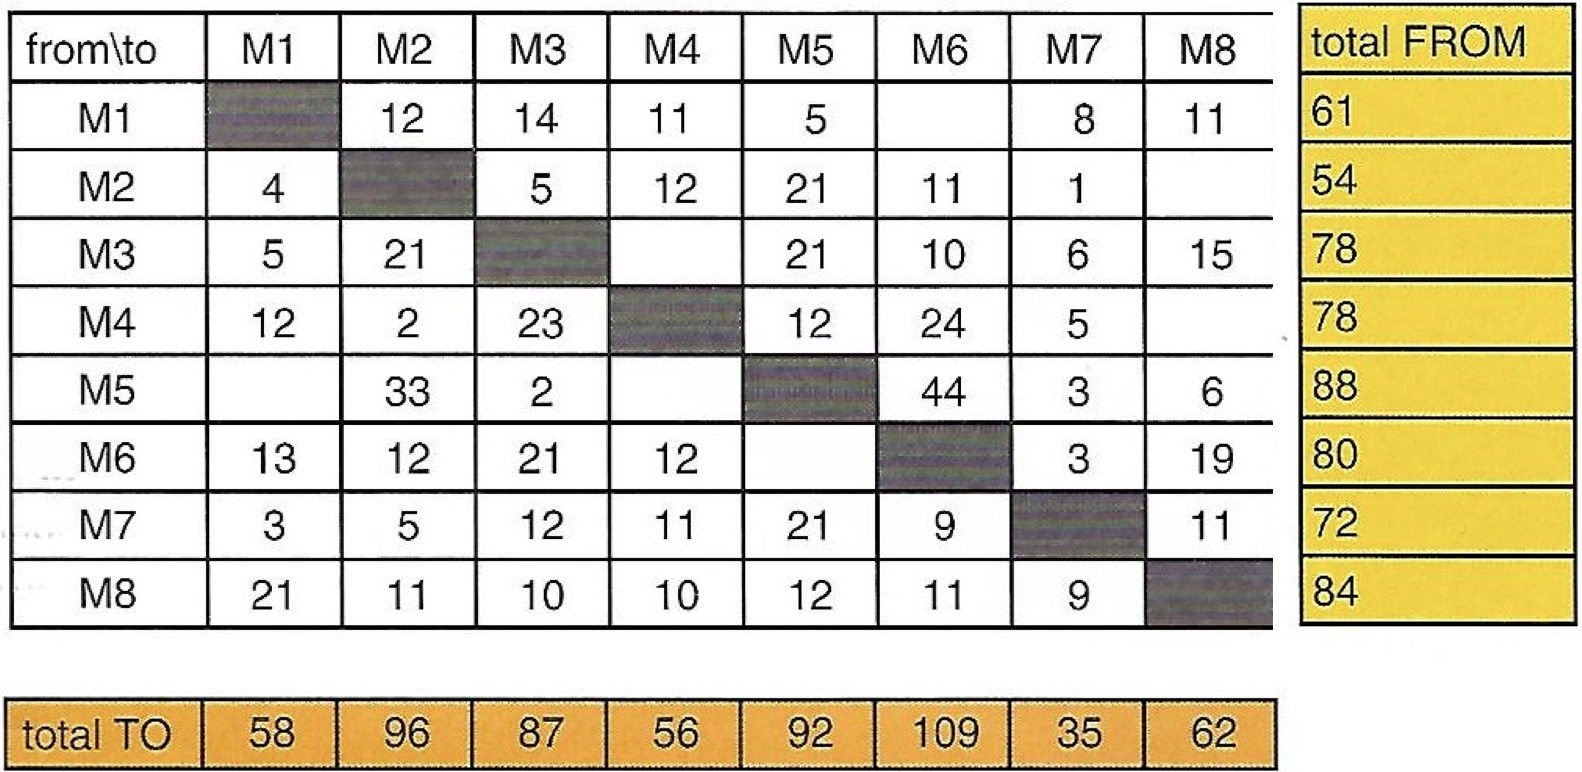
\includegraphics[width=\linewidth]{assets/Screenshot 2026-01-24 at 16.28.58.png}
        \caption{Matrice from/to}\label{fig:fromto_matrix}
    \end{subfigure}
    \begin{subfigure}{0.45\linewidth}
        \centering
        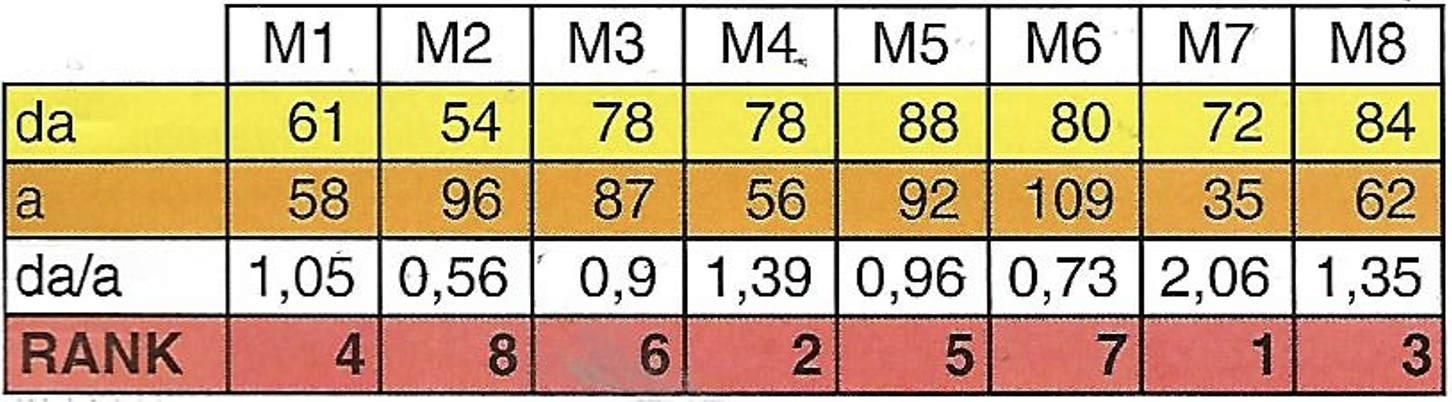
\includegraphics[width=\linewidth]{assets/Screenshot 2026-01-24 at 16.30.24.png}
        \caption{Rapporto $ r=\frac{\text{From}}{\text{To}} $}\label{fig:ratio_matrix}
    \end{subfigure}
    \begin{subfigure}{0.45\linewidth}
        \centering
        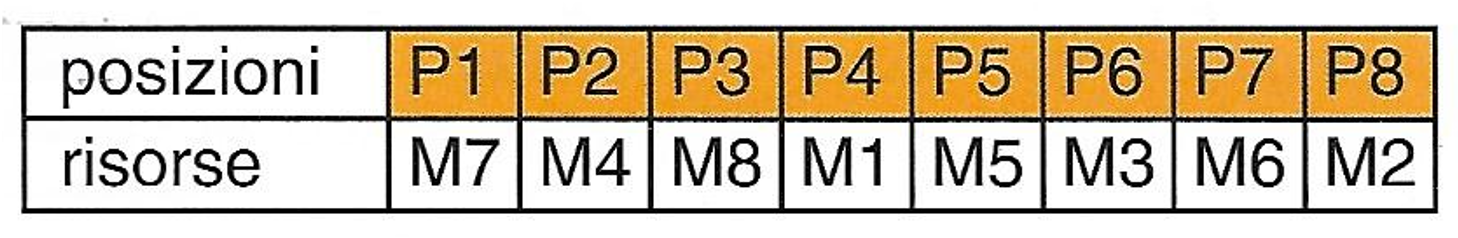
\includegraphics[width=\linewidth]{assets/Picture 5.png}
        \caption{Macchine ordinate}\label{fig:ordered_machines}
    \end{subfigure}
    \begin{subfigure}{0.45\linewidth}
        \centering
        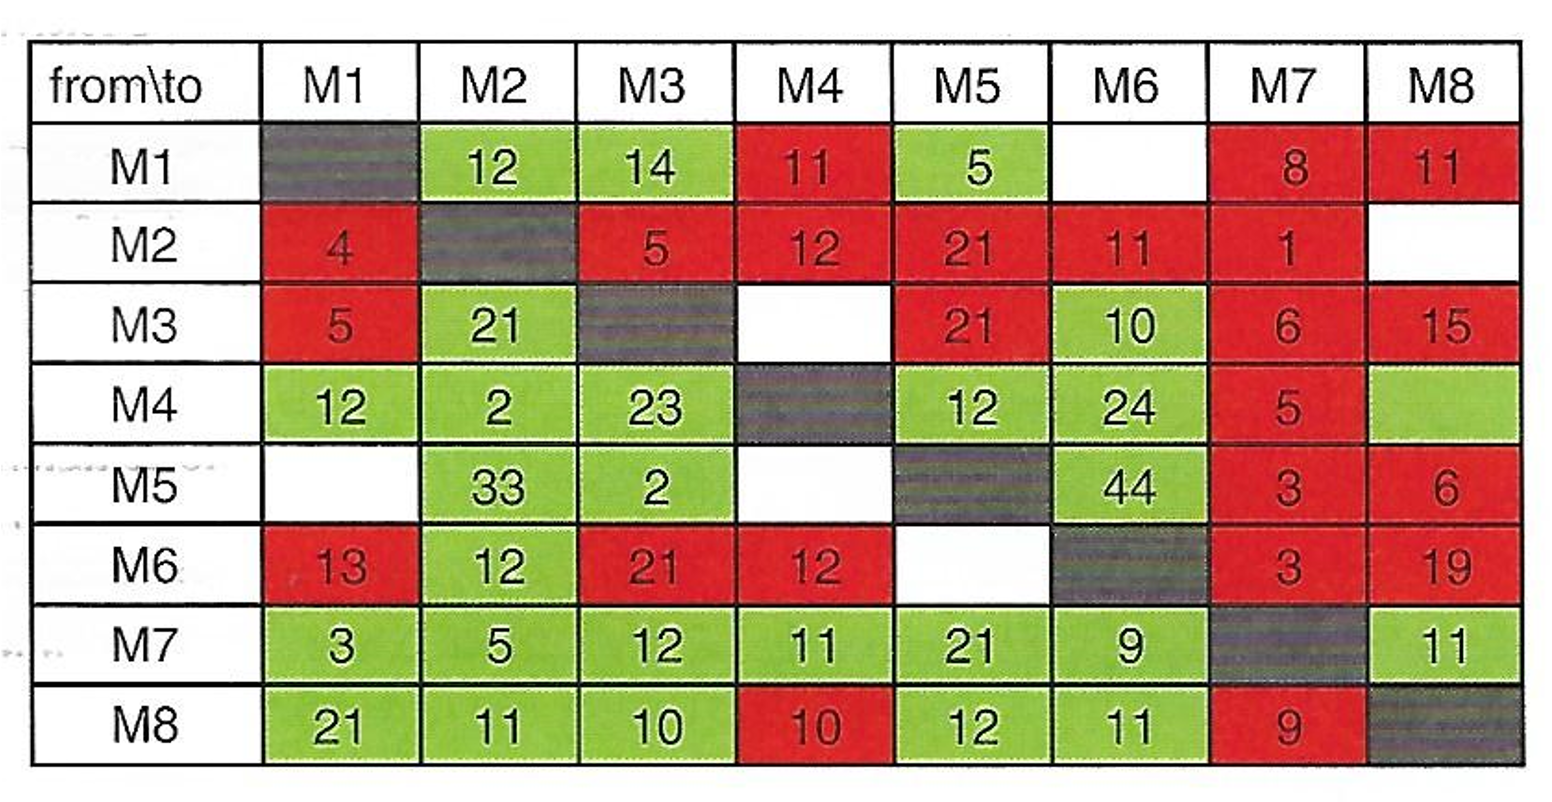
\includegraphics[width=\linewidth]{assets/Picture 6.png}
        \caption{Layout con flussi massimizzati}\label{fig:final_hollier}
    \end{subfigure}
    \caption{Metodo di Hollier}\label{fig:hollier}
\end{figure}

\subsubsection{Triangolo di Buffa} Uno strumento grafico per visualizzare le relazioni e le direzioni di trasporto tra reparti, utile per determinare le adiacenze prioritarie. Vedi figura \ref{fig:buffa_triangle}.
\begin{figure}
    \centering
    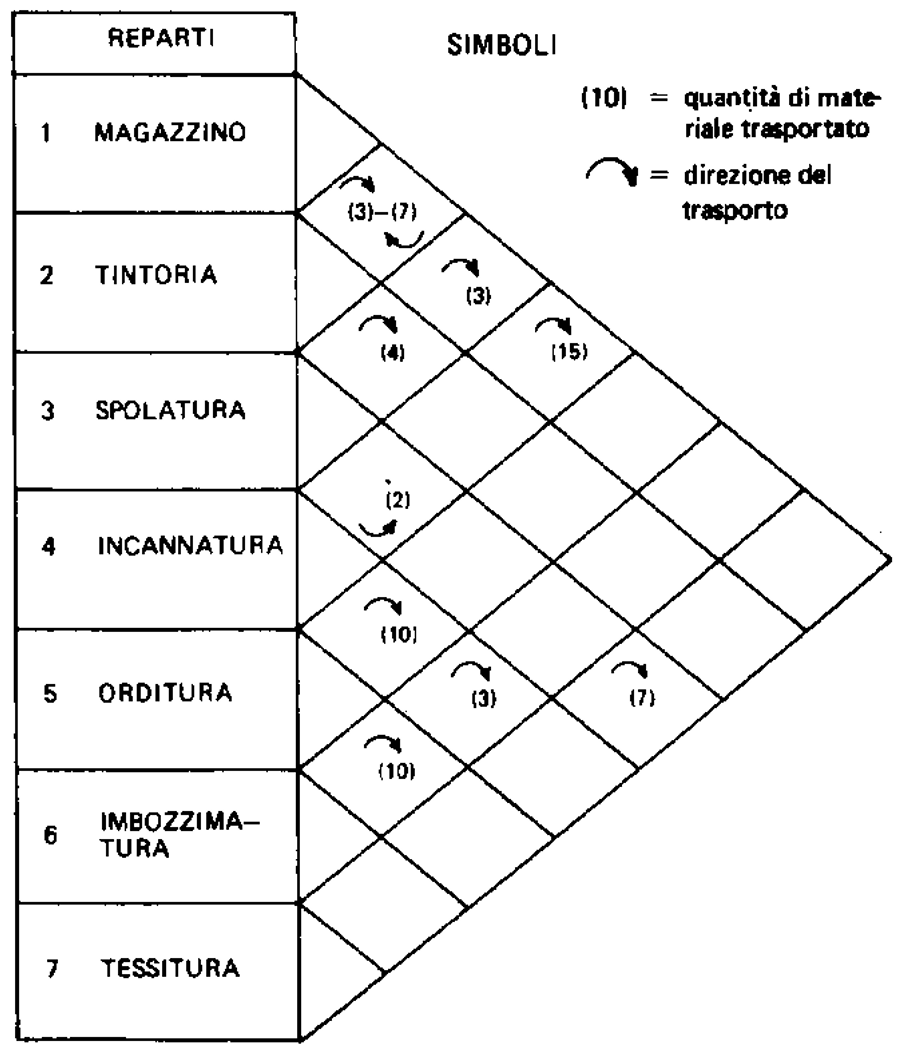
\includegraphics[width=0.35\linewidth]{assets/Picture 7.png}
    \caption{Triangolo di Buffa}\label{fig:buffa_triangle}
\end{figure}

%
\subsection{Configurazione finale} % chktex-file 17
Una volta definito lo schema logico, si sceglie la configurazione fisica considerando l'edificio e le future espansioni. Le principali configurazioni di layout sono:
\begin{itemize}
    \item Lineare: Espansione alle estremità, vedi figura \ref{fig:layout_lineare};
    \item Ad U: Ingresso e uscita vicini (banchine comuni), compatta, vedi figura \ref{fig:layout_adu};
    \item Ad L: Adattabile ad angoli dell'edificio, vedi figura \ref{fig:layout_adl}.
\end{itemize}

\begin{figure}
    \centering
    \begin{subfigure}{0.3\linewidth}
        \centering
        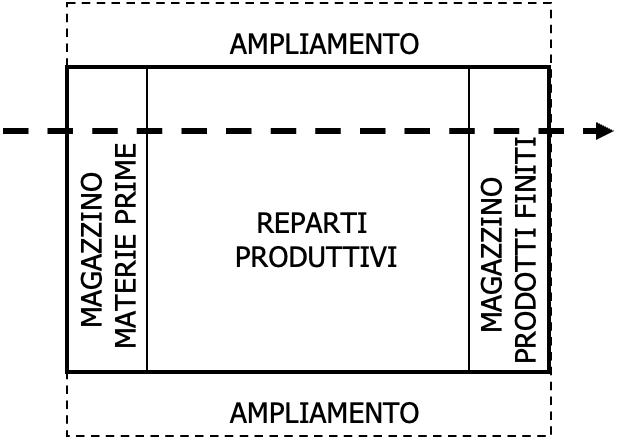
\includegraphics[width=\linewidth]{assets/Screenshot 2026-01-24 at 16.40.35.png}
        \caption{Layout lineare}\label{fig:layout_lineare}
    \end{subfigure}
    \begin{subfigure}{0.3\linewidth}
        \centering
        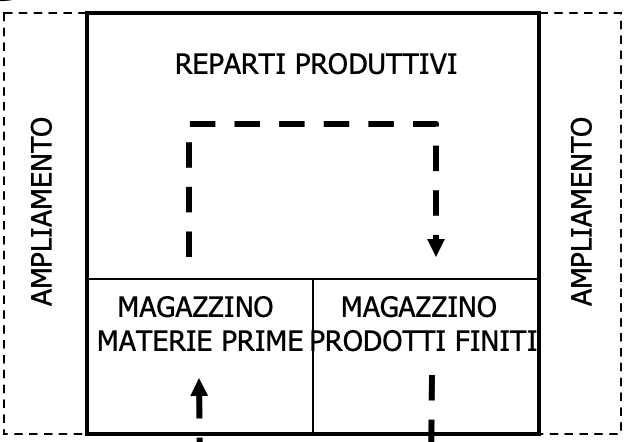
\includegraphics[width=\linewidth]{assets/Screenshot 2026-01-24 at 16.40.44.png}
        \caption{Layout ad U}\label{fig:layout_adu}
    \end{subfigure}
    \begin{subfigure}{0.3\linewidth}
        \centering
        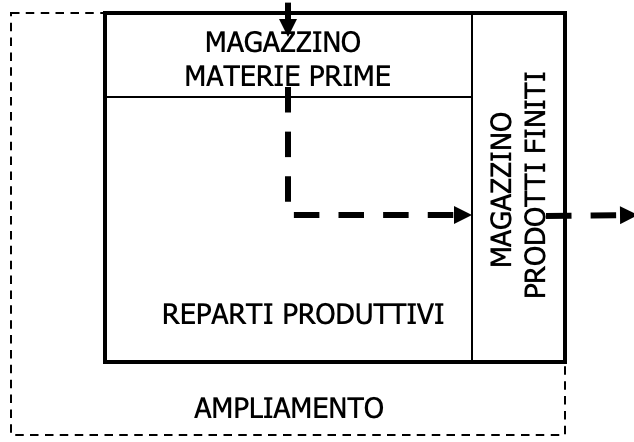
\includegraphics[width=\linewidth]{assets/Screenshot 2026-01-24 at 16.40.54.png}
        \caption{Layout ad L}\label{fig:layout_adl}
    \end{subfigure}
    \caption{Layouts di configurazione}\label{fig:layouts}
\end{figure}
%
\paragraph{Stesura del layout} Esistono software specifici (es. CATIA, CRAFT, CORELAP, FactoryFLOW \dots) per gestire problemi complessi che il calcolo manuale non può risolvere efficientemente.
\begin{itemize}
    \item \textbf{Stesura manuale}: Usa tecniche grafiche, lento su grandi dati, difficile comparare molte alternative.
    \item \textbf{Stesura computerizzata}: Calcoli veloci, gestisce numerosi reparti, integra algoritmi matematici, permette di valutare rapidamente diverse alternative.
\end{itemize}